\section{Experiments}
\label{sec:experiments}


\paragraph{Dataset} We use KITTI dataset for our experiments.  \cite{geiger2013vision}. KITTI dataset is a labeled video sequence of road scenes under variety of driving conditions including highways and residential areas in Karlsruhe, Germany. It provides manually labelled ground truth data for localization of cars and also uses velodyne data provide metrically accurate estimates of cars location.


%%%%%%%%%%%%%%%%%%%%%%%%%%%%%%%%%%%%%%%%%%%%%%%%%%%%
\subsection{Association error evaluation}

To verify the correctness of our association probability $\assocP$ we perform
association error experiment that compare the accuracy of point track
association with TPs with that of bounding box baseline method.

Note that the fraction $\assocP$ although called association probability does
not capture the entire information that we have available for compute
association of points to tracks. This above fraction is the association
probability given the hypothesized parameters of TP model. 

To compute the association probability between TP $i$ and
point track $j$ we must use re-projection error as well. When the association
$i$ and $j$ is right and the point of reflection is at depth $\lambda$ the
re-projection error must be zero \eqref{eq:reprojerror}, otherwise the error
becomes a measure of distance from the true solution.
The error terms can be converted to probability domain by considering the error
term as negative log of probability

\begin{align}
  P^{(ij)}_{\text{assoc by reproj}}(\lambda) = \frac{1}{Z}\exp(-\Ereproj(\lambda))
\end{align}

Using both the evidence terms we can write probability of association as
\begin{align}
  P^{(ij)}_{\text{assoc}} = \frac{1}{Z'}\int_0^{\infty} \assocP \exp(-\Ereproj(\lambda))d\lambda
  \label{eq:prob-assoc}
\end{align}

Once we have the probability of association we can compute the best possible
assignment of TP for each point. The points having very small association
probability are assigned to the background,
\begin{align}
  i^*_{j} = \argmin_{i} \int_0^\infty \assocP \Ereproj(\lambda) d\lambda
\end{align}

We use bounding box based assignment of point tracks to TPs as the baseline.
For the regions where the bounding boxes overlap, we assign the points to the
TP that has smaller mean depth then the competing bounding box.

\begin{figure*}
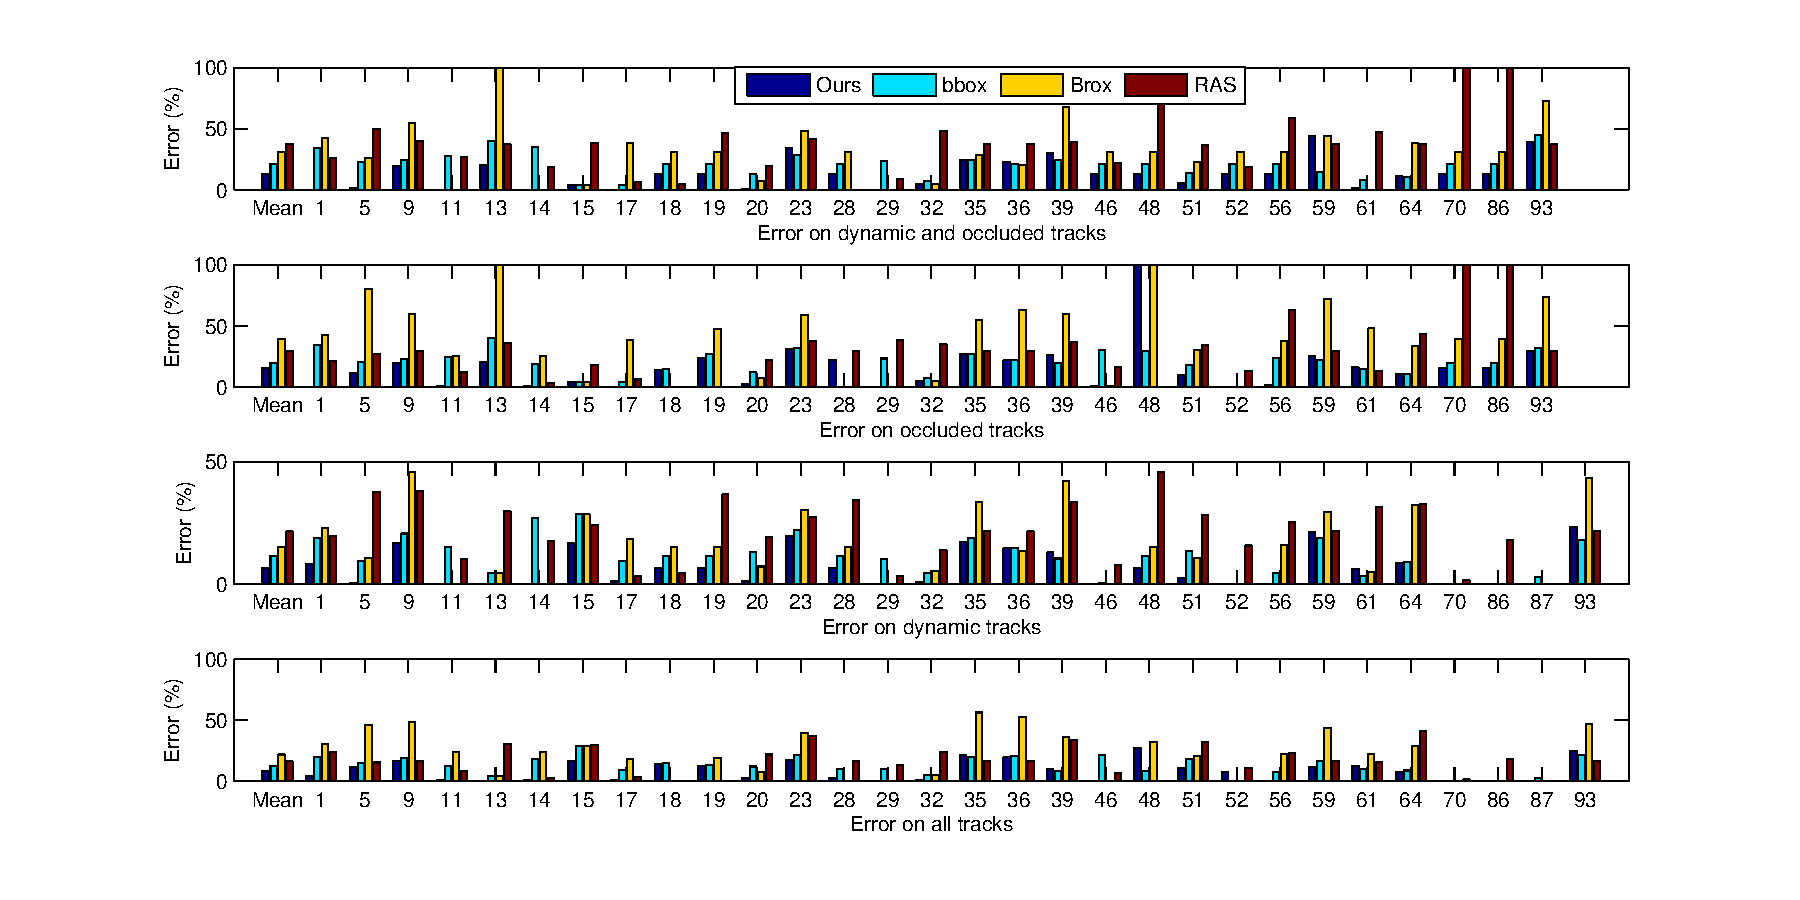
\includegraphics[trim=1.0in 0.4in 1.0in 0.2in, clip, width=\textwidth]{results/plotErrorBarEvalAssocCoeffAllSequence.pdf}
  \caption{Association error evaluation on different selection of tracks. The
    numbers on y-axis represent the data sequence number in KITTI dataset. The
    first set of bars in each plot correspond to the mean across all sequences.
    The error is in terms of average fraction of foreground points incorrectly
    associated to objects per sequence. Occluded points are chosen because our
    method is especially helpful in occlusion cases while dynamic points are
    chosen for fair comparison against motion segmentation methods.}
\label{fig:assoc-occ-results}
\end{figure*}


\newlength{\tblimgwidth}
\setlength{\tblimgwidth}{0.40\textwidth}
\begin{table*}
  \centering
  \begin{tabular}{ccc}
    & Associations & Error in association\\
    \rotatebox{90}{\hspace{2em} BBox} & 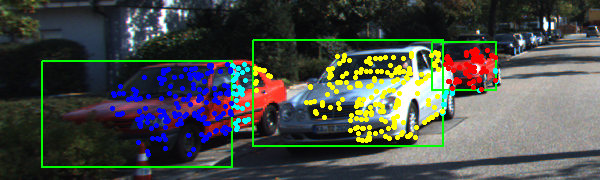
\includegraphics[width=\tblimgwidth]{results/0009_0000000060_point_assign_bbox2D_model-small.png} &%
    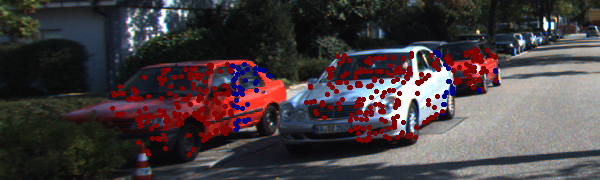
\includegraphics[width=\tblimgwidth]{results/0009_0000000060_point_assign_bbox2D_model_correct_incorrect-small.png}\\
    \rotatebox{90}{\hspace{2em} Brox} & 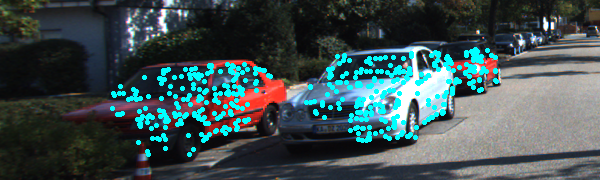
\includegraphics[width=\tblimgwidth]{results/0009_0000000060_point_assign_BroxAndMalik2010-small.png} &%
    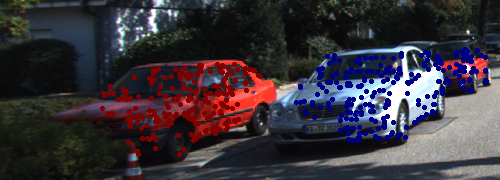
\includegraphics[width=\tblimgwidth]{results/0009_0000000060_point_assign_BroxAndMalik2010_correct_incorrect-small.png}\\
    \rotatebox{90}{\hspace{2em} RAS} & 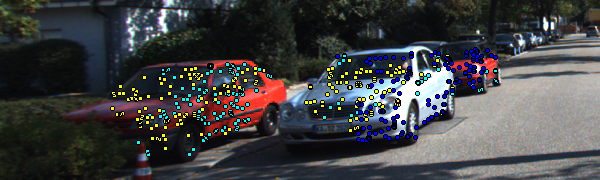
\includegraphics[width=\tblimgwidth]{results/0009_0000000060_point_assign_RAS-small.png} &%
    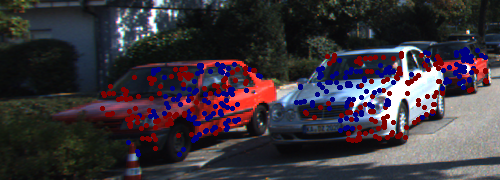
\includegraphics[width=\tblimgwidth]{results/0009_0000000060_point_assign_RAS_correct_incorrect-small.png}\\
    \rotatebox{90}{\hspace{2em} Ours} & 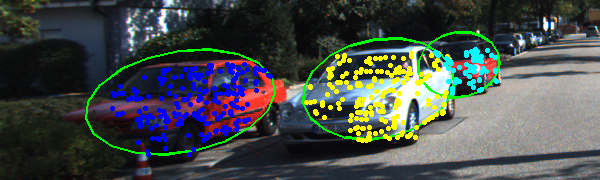
\includegraphics[width=\tblimgwidth]{results/0009_0000000060_point_assign_contPtTracks-small.png} &%
    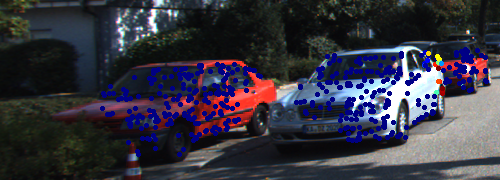
\includegraphics[width=\tblimgwidth]{results/0009_0000000060_point_assign_contPtTracks_correct_incorrect-small.png}\\
    \rotatebox{90}{\hspace{2em} BBox} & 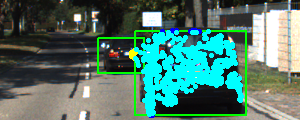
\includegraphics[width=\tblimgwidth]{results/0013_0000000060_point_assign_bbox2D_model-small.png} &%
    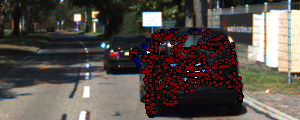
\includegraphics[width=\tblimgwidth]{results/0013_0000000060_point_assign_bbox2D_model_correct_incorrect-small.png}\\
    \rotatebox{90}{\hspace{2em} Brox} & 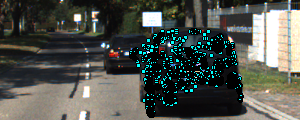
\includegraphics[width=\tblimgwidth]{results/0013_0000000060_point_assign_BroxAndMalik2010-small.png} &%
    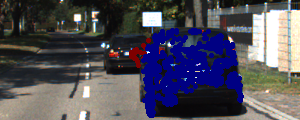
\includegraphics[width=\tblimgwidth]{results/0013_0000000060_point_assign_BroxAndMalik2010_correct_incorrect-small.png}\\
    \rotatebox{90}{\hspace{2em} RAS} & 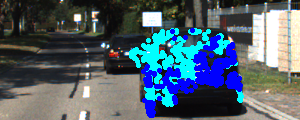
\includegraphics[width=\tblimgwidth]{results/0013_0000000060_point_assign_RAS-small.png} &%
    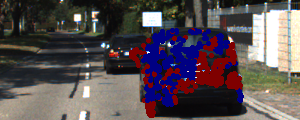
\includegraphics[width=\tblimgwidth]{results/0013_0000000060_point_assign_RAS_correct_incorrect-small.png}\\
    \rotatebox{90}{\hspace{2em} Ours} & 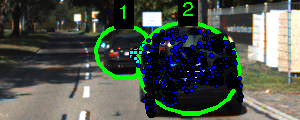
\includegraphics[width=\tblimgwidth]{results/0013_0000000060_point_assign_contPtTracks-small.png} &%
    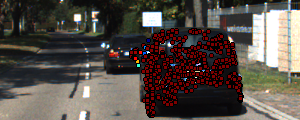
\includegraphics[width=\tblimgwidth]{results/0013_0000000060_point_assign_contPtTracks_correct_incorrect-small.png}
  \end{tabular}
  \caption{Qualitative results for association experiment. The left column
  shows the point tracks assignment to appropriate track. Each color represents
a different track to which the point is associated to. Right column shows the
probablistic error in association: red is low error and blue is high error.
Note that our method changes smoothly at the boundary of the objects with
intermediate probabilities, while the baseline methods have only 0-1 error.} 
\end{table*}


\subsection{Localization Experiment}
To show the effectiveness of our method we apply it to the localization
problem. We estimate the position, orientation and dimensions of the car with
our framework and compute the error in birds eye view domain along the ground
plane. We report error in three metrics translation error (t) in meters per
car, yaw error (yaw) in radians per car and dimension error is again meters per
car. The results are shown in Table~\ref{tab:localizationExperiment}.

We build the graphical model as shown in Fig~\ref{fig:graphmodel} that 
allows us to factorize the intractable probability distribution into following form
%
\begin{multline}
  -\log{P(\{\state{i}{t}\} | \mathbb{E})} = 
  -Z' 
  \\
  + \sum_{t=s_i}^{e_i}
  \left(
  \sum_{i,j:i\ne j}   
  \WEnergyCol 
   + \WpEnergy{bbox}
   + \WpEnergy{track}
\right)
  \\
  + \left(
  \sum_{i=1}^N 
  \WEnergy{lane}
  + \WEnergy{dyn}
  + \WEnergy{size}
\right)
  \enspace.
\end{multline}
%
We use the following energies in our graphical model.

\subsubsection{Continuous point tracks energy with occlusion}
\label{sec:totalContPtTracksEnergy}
We model continuous point tracks energy with explicit occlusion reasoning as
the expected re-projection error over the association probability,

\begin{multline}
  \Energy{track}(\{ \relp{i}{t} \}_i, \{ \relp{i}{t-1} \}_i, \{\dimsn{i}\}_i ) = 
  \\
    \sum_{i=1}^{N} 
    %\sum_{t = s_i}^{e_i}
    \sum_{j = 1}^{M}
    \int_1^\infty \assocP\Ereproj(\lambda) d\lambda
\end{multline}
where $\assocP$ is the association probability of
$j$\textsuperscript{th} point with $i$\textsuperscript{th} TP at depth $\lambda$, $\{ \relp{i}{t} \}_i$ are the poses of all occluding objects at time $t$, $ \{ \dimsn{i} \}_i$ are the dimensions of all objects that occlude $i$
and $\Ereproj(\lambda)$ is the re-projection error given by
%
\begin{align}
  \assocP &= \Prefl\Ptrans\\
  \Ereproj(\lambda) &= \left\|\trackpj{t} - \projectionOf{\invProjectionOftm{\trackpj{t-1}, \lambda}}\right\|^2 .
  \label{eq:reprojerror}
\end{align}

The  $\projectionOf{.}$ and $\invProjectionOftm{.}$ denote the projection and
inverse projection functions that project 3D point to camera image and vice
versa. Note that inverse projection $\invProjectionOf{.}$ depend on both the
point $\trackp{t}$ and the unknown depth $\lambda$. Also note that the inverse projection is dependent on TP pose at time $t-1$ while the projection depends on pose at time $t$ which can be different.

\subsubsection{Continuous bounding box energy with occlusion}

Object detection is usually followed by non-maximal suppression that results in
discarding similar bounding boxes. When we are jointly optimizing detections
with other cues, it is not usually desirable to go with a single bounding box.
Hence, we keep all the bounding box detections by approximating them with
multi-modal sum of Gaussian like logistic functions. We fit the parametric function of the form 
%
\begin{multline}
  S(\bb{i}) = \\
  \sum_k A_k \exp(-(\bb{i}-\mu^{(d)}_k)^\top \Sigma^{(d)-1}_k
  (\bb{i}-\mu^{(d)}_k))
\end{multline}
%
to detection scores, by non-linear error minimization with initialization from
non-maximal suppressed outputs. Here $\mu^{(d)}_j$ is one of the $k$ modes as a
4D vector representing a single bounding box as $[\minx, \miny, \maxx,
\maxy]^\top$. The optimization is constrained with symmetry and positive
definiteness of $\Sigma^{(d)-1}_k$, $\maxx \ge \minx$ and $\maxy \ge \miny$.

\paragraph{Detection scores with occlusion reasoning} 
\def\u{\mathbf{u}}
With our model of $\Ptrans$ described in Section \ref{sec:ptransmission}, we can
compute the probability of a point $\u$ on image be occluded assuming
the point is on traffic participant (TP) $i$ with mean depth $\mu^{(i)}_d$ as
\begin{align}
  O_{i}(\u, \mu^{(i)}_d) = 1 - \Ptransmission(\mu^{(i)}_d\u) \enspace .
\end{align}

If we know a portion of our proposed detection bounding box is known to be
occluded, then we would like to decrease the confidence in the detection score
about the localization of that end of the object. Assuming that the occlusion
is often on the boundary of detection bounding boxes, we want to decrease our
confidence on the mean detection boundaries around the occluded boundaries.
To re-model our detection scores scaled by continuous occlusion we sample
$O_{i}(\mathbf{u}, \mu^{(i)}_d)$ at the hypothesized detection boundaries from
GMM $S(.)$ and we augment the detection boundary covariance matrix by
$\mathcal{P}_{j} = \rho_{j}\rho_{j}^\top$ where $\rho_{j} = O_{j}(\mathbf{u},
\mu^{(i)}_d)$. The new covariance matrix in detection score is given by 
  $\Sigma'^{(d)}_j = \mathcal{P}_{j} + \Sigma^{(d)}_j$.
The detection scores GMM with occlusion is given by replacing the covariance
matrix
%
\begin{multline}
  S'(\bb{i}) =
  \\
  \sum_j A_j \exp(-(\bb{i}-\mu^{(d)}_j)^\top \Sigma'^{(d)-1}_j
  (\bb{i}-\mu^{(d)}_j))
\end{multline}

The energy of detection scores is simply take to be the inverse of the detection score.
\begin{align}
  \Energy{detect}(\{ \relp{i}{t} \}_i, \{ \relp{i}{t-1} \}_i, \{\dimsn{i}\}_i ) = \frac{1}{S'(\bb{i})}
\end{align}

For object detections we use object detector by \cite{Felzenszwalb_etal_2010}
which is detector by parts model and we use eight parts to train the car model 
on half of the KITTI dataset \cite{geiger2013vision}. The trained modeled is 
used to get detections for the other half of the dataset and vice versa. 

\subsubsection{Other energies}
Other energies we use are described in detail in the supplementary material. We briefly describe them here:
\begin{description}
  \item[Lane energy ($\Energy{lane}$)] This energy term constrains the
    orientation of traffic participants to be parallel to the nearest detected
    lane. The lanes are either detected visually or obtained from GPS and Map 
    information.
  \item[Transition probability ($\Energy{dyn}$)] We use these energies to
    constrain the motion of cars to be smooth in linear motion and rotation
    motion. We also constrain cars to move in the direction of heading.
  \item[Size prior ($\EnergySize$)] We use size prior of cars by using the mean
    of cars over the KITTI dataset.
\end{description}



\begin{figure}
  \centering
  \newcommand{\imagewidth}{\columnwidth}
  ../../CVPR/Source/scenelayoutoverlayCity0961.tex
  \caption{A sample road scene with the unknowns of each car modeled as random variables. 
  The relating energies are shown in Figure~\ref{fig:graphmodel}}
\end{figure}
\begin{figure}
    \usetikzlibrary{trees,shadows}
\begin{tikzpicture}[grow cyclic, line width=1.2pt,
    variablenode/.style={circle,circular drop shadow,draw=red,fill=white,thick,minimum width=0.5cm},
   bboxfactor/.style={rectangle,drop shadow,draw=green,fill=green,thick,minimum width=0.2cm},
    collfactor/.style={rectangle,drop shadow,draw=blue,fill=blue,thick,minimum width=0.2cm},
    trackfactor/.style={rectangle,drop shadow,draw=red,fill=red,thick,minimum width=0.2cm},
  obs/.style={fill=gray!30,draw=black},
  prevf/.style={draw=green!20,text=gray},
  prevobsv/.style={draw=gray!10,fill=gray!1,text=gray},
  prevv/.style={draw=red!20,text=gray}
]
  \path[use as bounding box,clip] (-2.5, -5.5) rectangle (5.5,0.5);
  \draw (-2.5,-2.65) rectangle +(0.5,0.3);
  \draw (-2.0,-2.35) -- ++(0.15, 0.15) -- ++(0, -0.6) -- (-2.0, -2.65);
\path
     (0, 0)  node [variablenode] (x6) {6}
++(0, -1.5) node [variablenode] (x2) {2}
++(2.5, 0)  node [variablenode] (x5) {5}
+ (0, 1.5)  node [variablenode,obs] (u) {}
+(.2,1.0)  node {$u$}
+ (.5, -2)   node [variablenode] (x3) {3}
+ (2.3, -3.5)   node [variablenode] (x4) {4}
+(2.5, 0)  node [variablenode] (x1) {1}
;

% Factors between nodes 6 and 2
\draw (x6) edge [bend right=35] node [bboxfactor] (f26) {} (x2);
\path (f26) +(-0.75,0) node [variablenode,obs] (d6) {} 
                        +(-.7,-.6)  node {$d^6$};
\draw (f26) edge (d6);
\draw (x6) edge [bend left=35] node [trackfactor] (ft26) {} (x2);
\draw (ft26) edge [bend left=10] (u);
\draw (x6) edge node [collfactor] {} (x2);

% Factors for node 2
\path (x2) +(0,-1.25) node [variablenode,obs] (d2) {} 
                        +(-.6,-1.3)  node {$d^2$};
\draw (x2) edge node [bboxfactor] {} (d2);

% Factors between nodes 2 and 5
\draw (x2) edge [bend right] node [bboxfactor] (f25) {} (x5);
\draw (x2) edge [bend left] node [trackfactor] (ft25) {} (x5);
\draw (x2) edge [] node [collfactor] {} (x5);
\draw (ft25) edge (u);
\path (x5) ++(-1.25,-1.25) node [variablenode,obs] (d5) {} 
                        +(.6,0)  node {$d^5$};
\draw (f25) edge (d5);

% Factors between nodes 5 and 1
\draw (x5) edge [bend right] node [bboxfactor] (f51) {} (x1);
\draw (x5) edge [bend left] node [trackfactor] (ft51) {} (x1);
\draw (x5) edge [] node [collfactor] {} (x1);
\draw (ft51) edge [bend right] (u);
\path (x1) ++(-1.25,-1.25) node [variablenode,obs] (d1) {} 
                        +(-.5,0.2)  node {$d^1$};
\draw (f51) edge (d1);

% Factors for node 3
\path (x3) ++(0,-1.25) node [variablenode,obs] (d3) {} 
                        +(.6,0)  node {$d^3$};
\draw (x3) edge node [bboxfactor] {} (d3);

% Factors for node 4
\path (x4) ++(0,1.25) node [variablenode,obs] (d4) {} 
                        +(.6,0)  node {$d^4$};
\draw (x4) edge node [bboxfactor] {} (d4);

% Legend
\path (-1.75,-4.0) node (l1s) {} (-0, -4.0) node [anchor=west] (l1e) {$\Energy{bbox}$};
\draw (l1s) edge node [bboxfactor] {} (l1e);
\path (-1.75,-4.5) node (l2s) {} (0, -4.5) node [anchor=west] (l2e) {$\EnergyCol$};
\draw (l2s) edge node [collfactor] {} (l2e);
\path (-1.75,-5.0) node (l3s) {} (0, -5.0) node [anchor=west] (l3e) {$\Energy{point}$};
\draw (l3s) edge node [trackfactor] {} (l3e);

\end{tikzpicture}

    \caption{Graphical model for a single frame with state of car represented
    as single node.  The six numbered nodes represent the unknown state variables of each car. The shaded nodes in the graphical model are observed variables. }
  \label{fig:graphmodel}
\end{figure}

\begin{table}
  \centering
  \begin{tabular}{lrrr}
    \toprule
    Energy & t & yaw & dim \\
    \midrule
    initialization                                                                                  & 3.79 & \textbf{0.86} & 1.64 \\
    $\EnergyLane+\EnergySize+\EnergyBBox+\EnergyDyn                                       $ & 3.83 & 0.90 & \textbf{1.14} \\
    %$\EnergyLane+\EnergySize+\EnergyBBoxocc+\EnergyDyn                                    $ & 3.83 & 0.90 & 1.14 \\
    %$\EnergyLane+\EnergySize+\EnergyBBoxocc+\EnergyDyn+\EnergyCol                         $ & 3.92 & 0.91 & 1.15 \\
    %$\EnergyLane+\EnergyContpttracks+\EnergySize+\EnergyBBoxocc+\EnergyDyn             $ & 3.81 & 0.92 & 1.59 \\
    % \EnergyBBox+\EnergyDyn+\EnergyCol $
    $\EnergyTrackNoOcc+\EnergyCol + \EnergyLane + \dots$  & 3.80 & 0.91 & 1.58 \\
    $\EnergyTrack+\EnergyCol + \EnergyLane + \dots$ & \textbf{3.78} & 0.91 & 1.58 \\
    \bottomrule
  \end{tabular}
  \caption{Localization experiment results with different combination of energies. We report error in three metrics translation error (t) in meters per car, yaw error (yaw) in radians per car and dimension error is again meters per car.}
  \label{tab:localizationExperiment}
\end{table}
